\documentclass[letterpaper,11pt]{article}

\usepackage{amsmath}
\usepackage{amssymb}
\usepackage[hmargin=1.25in,vmargin=1in]{geometry}
\usepackage{booktabs}
\usepackage{graphicx}
\usepackage{hyperref}
\usepackage{lmodern}
\usepackage{microtype}
\usepackage{pdflscape}
\usepackage{subcaption}

\title{Coursework 4: STAT 570}
\author{Philip Pham}
\date{\today}

\begin{document}
\maketitle

\begin{enumerate}
\item Consider the so-called Neyman-Scott problem in which
  $Y_{ij}\mid \mu_i,\sigma_2 \sim_{\mathrm{ind}}
  \mathcal{N}\left(\mu_i,\sigma^2\right), i=1,\ldots,n,j=1,2.$
  \begin{enumerate}
  \item Obtain the MLE of $\sigma^2$ and show that it is inconsistent. Why does
    this inconsistency arise in this example?

    \begin{description}
    \item[Solution:] The likelihood is
      \begin{align}
        L\left(\mu,\sigma\right)
        &= \prod_{i=1}^n \prod_{j=1}^2 \frac{1}{\sqrt{2\pi\sigma^2}}\exp\left(
          -\frac{1}{2\sigma^2}\left(Y_{ij} - \mu_i\right)^2
          \right) \nonumber\\
        &= \prod_{i=1}^n \frac{1}{2\pi\sigma^2}\exp\left(
          -\frac{1}{2\sigma^2}\left[
          \left(Y_{i1} - \mu_i\right)^2
          +\left(Y_{i2} - \mu_i\right)^2
          \right]
          \right),
          \label{eqn:p1_likelihood}
      \end{align}
      so the log-likelikehood is
      \begin{equation}
        l\left(\mu,\sigma\right) = -n\log\left(2\pi\right) -n\log\left(\sigma^2\right)
        - \frac{1}{2\sigma^2}\sum_{i=1}^n\left[
          \left(Y_{i1} - \mu_i\right)^2
          +\left(Y_{i2} - \mu_i\right)^2\right].
        \label{eqn:p1_log_likelihood}
      \end{equation}

      Taking the derivative with respect to $\sigma^2$, we have
      \begin{equation}
        \frac{\partial}{\partial\sigma^2}l\left(\mu, \sigma^2\right)
          = -\frac{n}{\sigma^2} +
          \frac{1}{2\left(\sigma^2\right)^2}\sum_{i=1}^n
          \left[
            \left(Y_{i1} - \mu_i\right)^2 +
            \left(Y_{i2} - \mu_i\right)^2\right].
          \label{eqn:p1_score_sigma2}
        \end{equation}

        Solving Equation \ref{eqn:p1_score_sigma2}, where
        $\frac{\partial}{\partial\sigma^2}l\left(\hat{\mu},
          \hat{\sigma}^2\right) = 0$, we have
        \begin{equation}
          \hat{\sigma}^2 = \frac{1}{2n}\sum_{i=1}^n
          \left[
            \left(Y_{i1} - \hat{\mu}_i\right)^2 +
            \left(Y_{i2} - \hat{\mu}_i\right)^2\right].
          \label{eqn:p1_sigma_hat}
        \end{equation}

        Taking the derivative of Equation \ref{eqn:p1_log_likelihood} with respect
        to $\mu_i$, we have
        \begin{equation}
          \frac{\partial}{\partial\mu_i}l\left(\mu, \sigma^2\right)
          =
          \frac{1}{\sigma^2}\left(Y_{i1} + Y_{i2} - 2\mu_i\right).
          \label{eqn:p1_score_mu_i}
        \end{equation}
        
        Solving Equation \ref{eqn:p1_score_mu_i}, where
        $\frac{\partial}{\partial\mu_i}l\left(\hat{\mu},
          \hat{\sigma}^2\right) = 0$, we have
        \begin{equation}
          \hat{\mu}_i = \frac{Y_{i1} + Y_{i2}}{2}.
          \label{eqn:p1_mu_i_hat}          
        \end{equation}

        Substituting Equation \ref{eqn:p1_mu_i_hat} into Equation
        \ref{eqn:p1_sigma_hat}, we have
        \begin{equation}
          \hat{\sigma}^2 = \frac{1}{n}\sum_{i=1}^n\left(\frac{Y_{i1} - Y_{i2}}{2}\right)^2.
          \label{eqn:p1_sigma_hat_solved}
        \end{equation}

        Taking the expected value of Equation \ref{eqn:p1_sigma_hat_solved}, we have
        \begin{align}
          \mathbb{E}\left[\hat{\sigma}^2\right]
          &= \frac{1}{4n}\sum_{i=1}^n \left(\mathbb{E}\left[Y_{i1}^2\right] + \mathbb{E}\left[Y_{i2}^2\right]
            - 2\mathbb{E}\left[Y_{i1}Y_{i2}\right]\right) \nonumber\\
          &= \frac{1}{4n}\sum_{i=1}^n \left(
            \left(\sigma^2 + \mu_i^2\right) + \left(\sigma^2 + \mu_i^2\right) - 2\mu_i^2
            \right) \nonumber\\
          &= \frac{\sigma^2}{2}.
        \end{align}
        Clearly,
        $\mathbb{E}\left[\hat{\sigma}^2\right] = \sigma^2/2 \nrightarrow
        \sigma^2$, so the estimator is not consistent.

        This is because the MLE estimate of $\sigma^2$ depends on
        $\mu_1,\ldots,\mu_n$, so the number of parameters being estimated
        increases with $n$. Thus, the model is not well-defined.
      \end{description}
    \item Derive the posterior distribution corresponding to the prior
      \begin{equation}
        \pi\left(\mu_1,\ldots,\mu_n,\sigma^2\right) \propto \sigma^{-n-2}
        \label{eqn:p1_prior}
      \end{equation}
      and show that
      \begin{equation}
        \mathbb{E}\left[\sigma^2 \mid Y\right] = \frac{1}{2(n-1)}\sum_{i=1}^n
        \frac{\left(Y_{i1}-Y_{i2}\right)^2}{2}.
      \end{equation}

      \begin{description}
      \item[Solution:] Using the likelihood in Equation \ref{eqn:p1_likelihood}
        and the prior in Equation \ref{eqn:p1_prior}. We have that
        \begin{equation}
          p\left(\mu, \sigma^2 \mid Y\right) \propto L\left(\mu, \sigma^2\right)\pi\left(
            \mu_1,\ldots,\mu_n,\sigma^2
          \right).
          \label{eqn:p1_posterior_propto}
        \end{equation}

        We have that
        \begin{align}
          p\left(Y\right)
          &= \int_{0}^\infty\int_{-\infty}^{\infty}\cdots\int_{-\infty}^{\infty}
          L\left(\mu, \sigma^2\right)\pi\left(\mu_1,\ldots,\mu_n,\sigma^2\right)\,\mathrm{d}\mu_1\cdots
            \mathrm{d}\mu_n\,\mathrm{d}\sigma^2 \nonumber\\
          &= \int_{0}^\infty \frac{1}{2^n\pi^n\left(\sigma^2\right)^{(3n + 2)/2}} \left(\pi\sigma^2\right)^{n/2}
            \prod_{i=1}^n \exp\left(-\frac{1}{4\sigma^2}\left(Y_{i1} - Y_{i2}\right)^2\right)
            \,\mathrm{d}\sigma^2 \nonumber\\
          &= \int_{0}^\infty \frac{1}{2^n\pi^{n/2}\left(\sigma^2\right)^{n + 1}}
            \exp\left(-\frac{1}{4\sigma^2}\sum_{i=1}^n \left(Y_{i1} - Y_{i2}\right)^2\right)
            \,\mathrm{d}\sigma^2 \nonumber\\
          &= -\frac{2^n}{\pi^{n/2}}\left(\sum_{i=1}^n \left(Y_{i1} - Y_{i2}\right)^2\right)^{-n}
            \int_\infty^0u^{n-1}\exp\left(-u\right)\,\mathrm{d}u \nonumber\\
          &= \frac{1}{\pi^{n/2}}\left(\sum_{i=1}^n \frac{\left(Y_{i1} - Y_{i2}\right)^2}{2}\right)^{-n}\Gamma(n).
            \label{eqn:p1_evidence}
        \end{align}
        Normalizing Equation \ref{eqn:p1_posterior_propto} with the evidence
        Equation \ref{eqn:p1_evidence}, we have the posterior
        \begin{equation}
          \tiny
          p\left(\mu, \sigma^2 \mid Y\right)
          =
          \frac{\left(\sigma^2\right)^{-(3n+2)/2}}{2^n\pi^{n/2}\Gamma(n)}
          \left(\sum_{i=1}^n \frac{\left(Y_{i1} - Y_{i2}\right)^2}{2}\right)^{n}
          \prod_{i=1}^n \prod_{j=1}^2 \exp\left(
            -\frac{1}{2\sigma^2}\left(Y_{ij} - \mu_i\right)^2
          \right).
          \label{eqn:p1_posterior}
        \end{equation}

        Marginalizing $\mu$ in Equation \ref{eqn:p1_posterior}, we get
        \begin{align}
          p\left(\sigma^2 \mid Y\right)
          &= \int_{-\infty}^\infty \cdots \int_{-\infty}^\infty
            p\left(\mu, \sigma^2 \mid Y\right)\,\mathrm{d}\mu_1\cdots\mathrm{d}\mu_n
            \label{eqn:p1_posterior_sigma2}\\
          &= \frac{\left(\sigma^2\right)^{-n-1}}{2^n\Gamma(n)}
            \left(\sum_{i=1}^n \frac{\left(Y_{i1} - Y_{i2}\right)^2}{2}\right)^{n}
            \exp\left(-\frac{1}{4\sigma^2}\sum_{i=1}^n\left(Y_{i1} - Y_{i2}\right)^2\right).
            \nonumber          
        \end{align}

        Taking the expectation over the distribution in Equation
        \ref{eqn:p1_posterior_sigma2}, we have that
        \begin{align}
          \mathbb{E}\left[\sigma^2 \mid Y\right]
          &= \int_{0}^\infty\sigma^2p\left(\sigma^2 \mid Y\right)\,\mathrm{d}\sigma^2 \nonumber\\
          &= \frac{1}{\Gamma(n)}\int_{0}^\infty\left(\frac{1}{4\sigma^2}
            \sum_{i=1}^n \left(Y_{i1} - Y_{i2}\right)^2\right)^{n}
            \exp\left(-\frac{1}{4\sigma^2}\sum_{i=1}^n\left(Y_{i1} - Y_{i2}\right)^2\right) \nonumber\\
          &= \frac{\sum_{i=1}^n\left(Y_{i1} - Y_{i2}\right)^2}{4\Gamma(n)}
            \int_{0}^\infty u^{n-1-1}\exp\left(u\right)\,\mathrm{d}u
            \nonumber\\
          &=\frac{\Gamma(n-1)}{2\Gamma(n)}\sum_{i=1}^n\frac{\left(Y_{i1} - Y_{i2}\right)^2}{2} \nonumber\\
          &= \frac{1}{2(n-1)}\sum_{i=1}^n\frac{\left(Y_{i1} - Y_{i2}\right)^2}{2},
            \label{eqn:p1_posterior_sigma2_expectation}
        \end{align}
        which is the desired result.
      \end{description}
    \item Hence, using Equation \ref{eqn:p1_posterior_sigma2_expectation}, show
      that $\mathbb{E}\left[\sigma^2\mid Y\right] \rightarrow \sigma^2/2$ as
      $n\rightarrow\infty$, so that the posterior mean is inconsistent.

      \begin{description}
      \item[Solution:] From Equation \ref{eqn:p1_posterior_sigma2_expectation},
        we have that
        \begin{align}
          \lim_{n\rightarrow\infty} \mathbb{E}\left[\sigma^2\mid Y\right]
          &= \lim_{n\rightarrow\infty}
          \frac{1}{2(n-1)}\sum_{i=1}^n
          \frac{\mathbb{E}\left[\left(Y_{i1} - Y_{i2}\right)^2\right]}{2} \nonumber\\          
          &= \lim_{n\rightarrow\infty}
          \frac{1}{2(n-1)}\sum_{i=1}^n
            \frac{\operatorname{Var}\left(Y_{i1} - Y_{i2}\right)}{2} \nonumber\\
          &= \lim_{n\rightarrow\infty} \frac{n\sigma^2}{2(n-1)} \nonumber\\
          &= \frac{\sigma^2}{2} \neq \sigma^2,
        \end{align}
        so the posterior mean is inconsistent.
      \end{description}
    \item Examine the posterior distribution corresponding to the prior
      \begin{equation}
        \pi\left(\mu_1,\ldots,\mu_n\sigma^2\right) \propto \sigma^{-2}.
        \label{eqn:p1_prior2}
      \end{equation}

      \begin{description}
      \item[Solution:] If we use Equation \ref{eqn:p1_prior2}, Equation
        \ref{eqn:p1_evidence} becomes
        \begin{align}
          p\left(Y\right)
          &= \int_{0}^\infty \frac{1}{2^n\pi^{n/2}\left(\sigma^2\right)^{n/2+1}}
            \exp\left(-\frac{1}{4\sigma^2}\sum_{i=1}^n \left(Y_{i1} - Y_{i2}\right)^2\right)
            \,\mathrm{d}\sigma^2 \nonumber\\
          &= \frac{\Gamma\left(\frac{n}{2}\right)}{\pi^{n/2}}
            \left(\sum_{i=1}^n \left(Y_{i1} - Y_{i2}\right)^2\right)^{-n/2}.
            \label{eqn:p1_evidence2}
        \end{align}
        With Equation \ref{eqn:p1_evidence2}, the posterior becomes
        \begin{equation}
          \tiny
          p\left(\mu, \sigma^2 \mid Y\right)
          =
          \frac{\left(\sigma^2\right)^{-n-1}}{2^n\pi^{n/2}\Gamma(n/2)}
          \left(\sum_{i=1}^n \frac{\left(Y_{i1} - Y_{i2}\right)^2}{2}\right)^{n}
          \prod_{i=1}^n \prod_{j=1}^2 \exp\left(
            -\frac{1}{2\sigma^2}\left(Y_{ij} - \mu_i\right)^2
          \right).
          \label{eqn:p1_posterior2}
        \end{equation}

        Marginalizing Equation \ref{eqn:p1_posterior2} over $\mu$, we have
        \begin{equation}
          \scriptsize
          p\left(\sigma^2 \mid Y\right)
          = \frac{1}{\sigma^2\Gamma\left(n/2\right)}
          \left(\frac{\sum_{i=1}^n \left(Y_{i1} - Y_{i2}\right)^2}{4\sigma^2}\right)^{n/2}
          \exp\left(-\frac{\sum_{i=1}^n \left(Y_{i1} - Y_{i2}\right)^2}{4\sigma^2}\right).
          \label{eqn:p1_posterior_sigma22}
        \end{equation}
        Equation \ref{eqn:p1_posterior_sigma22} is quite similar to Equation
        \ref{eqn:p1_posterior_sigma2}, but with $n$ replaced by $n/2$ in the
        gamma function and the exponent of the sum of squares.        
      \end{description}
    \item Is the posterior mean for $\sigma^2$ consistent in this case?
      \begin{description}
      \item[Solution:] Yes. Taking the expectation with Equation
        \ref{eqn:p1_posterior_sigma22}, we have
        \begin{align}
          \mathbb{E}\left[\sigma^2 \mid Y\right]
          &= \int_0^\infty p\left(\sigma^2 \mid Y\right)\,\mathrm{d}\sigma^2\nonumber\\
          &= \frac{1}{4\Gamma\left(n/2\right)}\sum_{i=1}^n \left(Y_{i1} - Y_{i2}\right)^2
            \int_0^\infty  u^{n/2 - 1 - 1}\exp\left(-u\right)\,\mathrm{d}u
            \nonumber\\
          &= \frac{\Gamma\left(n/2 - 1\right)}{4\Gamma\left(n/2\right)}\sum_{i=1}^n \left(Y_{i1} - Y_{i2}\right)^2
            \nonumber\\
          &= \frac{1}{2\left(n/2 - 1\right)}\sum_{i=1}^n \frac{\left(Y_{i1} - Y_{i2}\right)^2}{2} \nonumber\\
          &= \frac{1}{n-2}\sum_{i=1}^n \frac{\left(Y_{i1} - Y_{i2}\right)^2}{2}.
            \label{eqn:p1_posterior_sigma2_expectation2}
        \end{align}

        Taking the limit of Equation \ref{eqn:p1_posterior_sigma2_expectation2},
        we have
        \begin{align}
          \lim_{n\rightarrow\infty}\mathbb{E}\left[\sigma^2 \mid Y\right]
          &= \lim_{n\rightarrow\infty} \frac{1}{n-2}\sum_{i=1}^n \frac{\mathbb{E}\left[
            \left(Y_{i1} - Y_{i2}\right)^2\right]}{2}
            \nonumber\\
          &= \lim_{n\rightarrow\infty} \frac{n}{\left(n-2\right)}
            \frac{1}{n}\sum_{i=1}^n \frac{\operatorname{Var}\left(Y_{i1} - Y_{i2}\right)}{2} \nonumber\\
          &= \lim_{n\rightarrow\infty} \frac{n}{\left(n-2\right)}
            \frac{1}{n}\sum_{i=1}^n \frac{2\sigma^2}{2} \nonumber\\
          &= \lim_{n\rightarrow\infty} \frac{n}{\left(n-2\right)}\sigma^2 \nonumber\\
          &= \sigma^2,
        \end{align}
        so the posterior mean is consistent when the prior doesn't depend on $n$.
      \end{description}
    \end{enumerate}
  \item The data in Table \ref{tab:p2_data} contain data on a typical
    reliability experiment and give the failure stresses (in GPa) of four
    samples of carbon fibers of lengths 1, 10, 20 and 50mm.

    \begin{table}
      \centering
      \tiny
      \begin{tabular}{rrrrrrrrrrrrrr}
\toprule
 Length (mm) &      0 &      1 &      2 &      3 &      4 &      5 &      6 &      7 &      8 &      9 &     10 &     11 &     12 \\
\midrule
           1 &  2.247 &  2.640 &  2.842 &  2.908 &  3.099 &  3.126 &  3.245 &  3.328 &  3.355 &  3.383 &  3.572 &  3.581 &  3.681 \\
          10 &  1.901 &  2.132 &  2.203 &  2.228 &  2.257 &  2.350 &  2.361 &  2.396 &  2.397 &  2.445 &  2.454 &  2.454 &  2.474 \\
          20 &  1.312 &  1.314 &  1.479 &  1.552 &  1.700 &  1.803 &  1.861 &  1.865 &  1.944 &  1.958 &  1.966 &  1.997 &  2.006 \\
          50 &  1.339 &  1.434 &  1.549 &  1.574 &  1.589 &  1.613 &  1.746 &  1.753 &  1.764 &  1.807 &  1.812 &  1.840 &  1.852 \\
\bottomrule
\end{tabular}

      \caption{Failure stress data for four groups of fibers.}
      \label{tab:p2_data}
    \end{table}

    \begin{enumerate}
    \item Consider a Bayesian analysis with an exponential likelihood and a
      gamma prior, $\lambda \sim \operatorname{Gamma}(a,b)$. Derive the form of
      the posterior distribution for $\lambda$.

      \begin{description}
      \item[Solution:] Suppose that we observe independent and identically
        distributed $Y_i \sim \operatorname{Exponential}(\lambda)$ for
        $i = 1,\ldots,n$. Let $Y = \left(Y_1,\ldots,Y_n\right)$. Then, we have
        the likelihood function
        \begin{equation}
          L(\lambda) = p\left(Y\mid\lambda\right) = \lambda^n\exp\left(
            -\lambda\sum_{i=1}^nY_i
          \right).
          \label{eqn:p2_likelihood}
        \end{equation}

        From Equation \ref{eqn:p2_likelihood}, we have the posterior
        \begin{align}
          p\left(\lambda \mid Y\right)
          &\propto p\left(Y\mid\lambda\right)p\left(\lambda\right) \nonumber\\
          &\propto \left(
            \lambda^n\exp\left(
            -\lambda\sum_{i=1}^nY_i
            \right)
            \right)
            \left(
            \frac{b^a}{\Gamma(a)}\lambda^{a - 1}\exp\left(-b\lambda\right)
            \right) \nonumber\\
          &\propto \lambda^{a + n - 1}\exp\left(
            -\left(b + \sum_{i=1}^nY_i\right)\lambda
            \right),
            \label{eqn:p2_posterior_propto}
        \end{align}
        which equal to the Gamma probability density function up to a constant
        factor independent of $\lambda$. Thus, we have that $\lambda \mid Y \sim
        \Gamma\left(a + n, b + \sum_{i=1}^nY_i\right)$, and
        \begin{equation}
          p\left(\lambda \mid Y \right)
          = \frac{\left(b + \sum_{i=1}^nY_i\right)^{a+n}}{\Gamma\left(a + n\right)}
          \lambda^{a + n - 1}\exp\left(-\left(b + \sum_{i=1}^nY_i\right)\lambda\right).
          \label{eqn:p2_posterior}
        \end{equation}
      \end{description}
    \item Choose $a$ and $b$ so that the prior probability that $\lambda$ lies
      between 0.05 and 1 is 0.95.
      \label{part:p2_prior}
      \begin{description}
      \item[Solution:] For a specified mean $\mu$, we specify our prior as the
        gamma distribution $\operatorname{Gamma}\left(k\mu,k\right)$ for some
        $k$. Let $F$ be the cumulative distribution function. We choose $k$ such
        that
        \begin{equation}
          F\left(1\right) - F\left(0.05\right) = 0.95.
          \label{eqn:p2_hyperparameter_equation}
        \end{equation}

        Choosing $a \approx 3.634$ and $b \approx 7.268$ satisfies Equation
        \ref{eqn:p2_hyperparameter_equation}. These values were obtained
        numerically in
        \href{https://nbviewer.jupyter.org/github/ppham27/stat570/blob/master/hw4/failure\_stresses.ipynb}{\texttt{failure\_stresses.ipynb}}.
      \end{description}
    \item Obtain the posterior means and posterior standard deviations for
      $\lambda$ and give histogram representations of
      $p\left(\lambda\mid y\right)$ for each of the groups in Table
      \ref{tab:p2_data}. Compare inference with the frequentist analyses.  Also
      give histogram representations of the posterior for $\lambda^{-1}$, again
      for each of the four groups.
      \begin{description}
      \item[Solution:] The posterior parameters, means, and standard deviations
        can be seen in Table \ref{tab:p2_gamma_posteriors}. The first two
        columns are the shape and rate parameters of the gamma posterior,
        respectively.        

        \begin{table}
          \centering
          \begin{tabular}{rrrrr}
\toprule
 Length (mm) &  $a^\prime$ &  $b^\prime$ &      Mean &  Standard error \\
\midrule
           1 &   16.634063 &   48.275125 &  0.344568 &        0.084484 \\
          10 &   16.634063 &   37.320125 &  0.445713 &        0.109284 \\
          20 &   16.634063 &   30.025125 &  0.554005 &        0.135836 \\
          50 &   16.634063 &   28.940125 &  0.574775 &        0.140928 \\
\bottomrule
\end{tabular}

          \caption{The results of updating the prior belief in Part
            \ref{part:p2_prior} with the data.}
          \label{tab:p2_gamma_posteriors}
        \end{table}

        The means are similar to the estimates from frequentist analyses in the
        previous homework but are drawn towards the prior mean of 0.5. The
        standard errors are slightly smaller tahn those obtained from fitting
        the exponential model but are much larger than either the
        quasi-likelihood model or sandwich estimates.

        For the posterior distribution of $\lambda^{-1}$, we have that
        \begin{align}
          p\left(\lambda^{-1} \mid Y\right)
          &= p\left(\lambda \mid Y\right)\left\lvert
            \frac{\mathrm{d}}{\mathrm{d}\lambda^{-1}}\left(\lambda^{-1}\right)^{-1}
          \right\rvert = p\left(\lambda \mid Y\right)\lambda^{2} \nonumber\\
          &= \frac{\left(b + \sum_{i=1}^nY_i\right)^{a+n}}{\Gamma\left(a + n\right)}
          \lambda^{a + n + 1}\exp\left(-\left(b + \sum_{i=1}^nY_i\right)\lambda\right),
          \label{eqn:p2_posterior_inverse}
        \end{align}
        where we used Equation \ref{eqn:p2_posterior} and transformation of
        random variables, so
        $\lambda^{-1} \mid Y \sim \operatorname{InverseGamma}\left(
          a + n,
          b + \sum_{i=1}^nY_i
        \right)$.

        Theoretical histograms along with their density are plotted in Figure
        \ref{fig:p2_posterior_lambda_inverse}.

        \begin{figure}
          \centering
          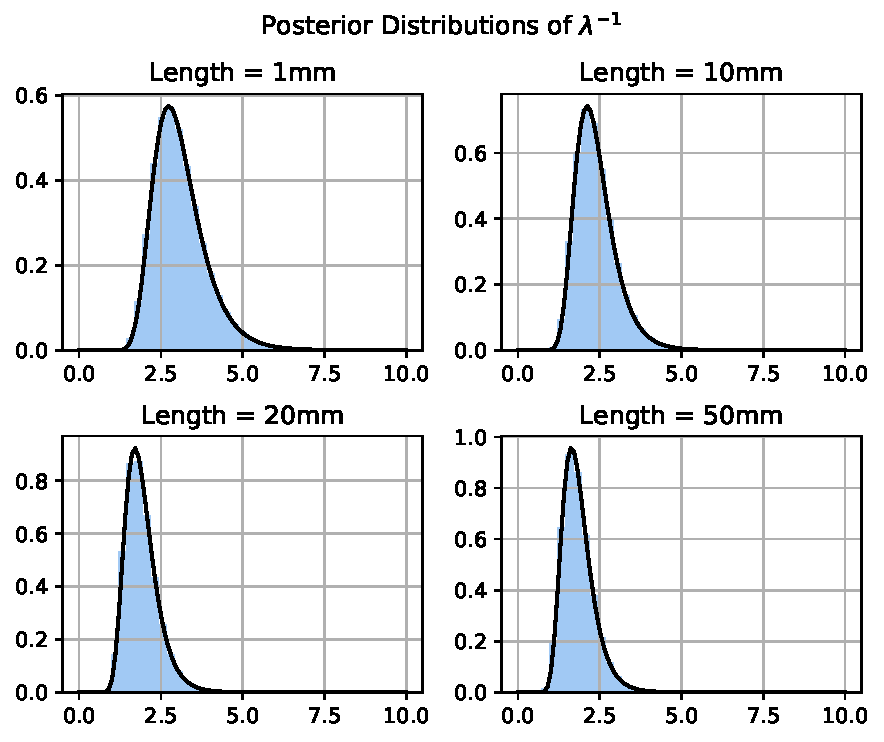
\includegraphics{p2_posterior_lambda_inverse.pdf}
          \caption{Histograms and probability density for samples drawn from the
            posteriors for $\lambda^{-1}$.}
          \label{fig:p2_posterior_lambda_inverse}
        \end{figure}

        Unlike the MLE, the posterior mean is not invariant under
        reparameterization:
        \[
          \mathbb{E}\left[\lambda^{-1} \mid Y\right] = \frac{b^\prime}{a^\prime - 1}
          \gneq  \frac{b^\prime}{a^\prime} = \frac{1}{\mathbb{E}\left[\lambda \mid Y\right]}.
        \]

        See
        \href{https://nbviewer.jupyter.org/github/ppham27/stat570/blob/master/hw4/failure\_stresses.ipynb}{\texttt{failure\_stresses.ipynb}} for code to reproduce plots.
      \end{description}
    \end{enumerate}
  \end{enumerate}
\end{document}
